In this chapter, a new constrained de Bruijn sequences are introduced. Since a de Bruijn sequence is self-located, the run length limited constraint is the only one requirement remain that this sequence needs to satisfy to be used in the \gls{dBTS} system. Therefore, combining a positioning sequence and a run length limited sequence is natural solution. That is also how this thesis gave birth to the name: Run length limited de Bruijn sequence. Beside, just like other constrained code, a convenient way to apprehend a code is using a labeled graph. Hence, the graph presentation of theses sequences is also provided. 

\section{Run Length Limited De Bruijn Sequence}

Let $n,k,s,q$ be some positive integers and $\Sigma_{q} = \left\{0,1,2,\ldots,q-1\right\}$ be an alphabet of size $q$. A \emph{sequence} $\bfs=\left(s_{1},s_{2},\ldots,s_{n}\right)\in\Sigma^{n}_{q}$ is over an alphabet $\Sigma$, that is, $s_{i}\in\Sigma_{q}$. This thesis only focuses on the case $q=2$ and thus drops $q$ in the notation for simplicity. Sequence $\bfs=s_{1}s_{2}\ldots s_{n}\in\Sigma^{n}$ is also written without ambiguity. The window (substring) $(s_{i},s_{i+1},\ldots,s_{j})$ is denoted by $s[i,j]$. 

Given two sequences $\bfx=x_{1}x_{2}\ldots x_{m}$ and $\bfy=y_{1}y_{2}\ldots y_{n}$, denote the concatenation of $\bfx$ and $\bfy$ to be $\bfx\bfy $ $=x_{1}x_{2}\ldots x_{m}y_{1}y_{2}\ldots y_{n}$, and denote $\bfx^{k}$ the concatenation of $k$ copies of $\bfx$. It is said that $\bfx$ is smaller than $\bfy$, denoted $\bfx<\bfy$, if there is an index $t\geq1$, such that $x_{i}=y_{i}$, $\forall i\leq t$, and $x_{t+1}<y_{t+1}$. Note that empty sequence is smaller than $0$.

\begin{definition}
    A  sequence $\bfs = (s_1,s_2,\ldots,s_n)$ is called a $s$-run length limited (RLL) sequence of length $n$ if each run of 0's in the sequence $\bfs$ has length at most $s$, or in other words, the sequence $\bfs$ does not contain $s+1$ consecutive 0's as a substring. 
A set of $s$-RLL sequences of length $n$ is called a $s$-RLL code and denoted $C(n,s)$.
\end{definition}

Denote $W(n,s)$ the set of all $s$-RLL sequences of length $n$ and note that $W(n,s)$ is the maximal $s$-RLL code. The $s$-RLL code $C(n,s)$ and the cardinality $|W(n,s)|$ has been well-studied in the literature~\cite{blake1982enumeration, kurmaev2011constant}. This thesis presents the recursive formula of $\card{W(n,s)}$ with proof.

\begin{lemma}[Cardinality of $W(n,s)$]\label{lem:card_W}
    Let $n,s$ be two non-negative integers. Then
    \begin{align*}
        \lvert W(n,s) \rvert &= 2^{s},\ \forall 0\leq n\leq s \\
        \lvert W(n,s) \rvert &= \sum_{i=0}^{s} \lvert W(n-i-1,s)\rvert,\ \forall n>s
    \end{align*}
\end{lemma}
\begin{proof}
    For the first equation, when $n\leq s$, all sequences of length $n$ belong to $W(n,s)$. Hence $\lvert W(n,s) \rvert = 2^{n},\ \forall 0\leq n\leq s$. 
    
    When $n>s$, every sequence in $W(n,s)$ is of the form $0^{i}1\bfx$, where $\bfx \in W(n-i-1,s)$ for $0 \leq i \leq s$. Additionally, for every $\bfx\in W(n-i-1,s)$, the sequence $0^{i}1\bfx$ is an element of $W(n,s)$. This bijection brings the second equation.
\end{proof}

% The very first values of $\card{W(n,s)}$ are listed in table~\ref{tab:values_of_W}. The first row includes values of $n$, while the first column contains the value of $s$. The crossed cell of column $n=i$ and row $s=j$ holds value of $\card{W(i,j)}$. 
Table~\ref{tab:values_of_W} lists the very first values of $\card{W(n,s)}$. Each $\card{W(i,j)}$ is stored at the crossed cell of column $n=i$ with row $s=j$.
\begin{table}[htbp]
    \centering
    \caption{Values of $W(n,s)$ for all $n=\overline{0,12}$ and $s=\overline{1,9}$.}
    \begin{tabular}{|c|c|c|c|c|c|c|c|c|c|c|c|c|c|c|c|c|}
    \hline
        \diagbox{s}{n} & 0 & 1 & 2 & 3 & 4 & 5 & 6 & 7 & 8 & 9 & 10 & 11 & 12\\
        % \hline\hline
        \hline
        1 & 1 & 2 & 3 & 5 & 8 & 13 & 21 & 34 & 55 & 89 & 144 & 233 & 377\\
        2 & 1 & 2 & 4 & 7 & 13 & 24 & 44 & 81 & 149 & 274 & 504 & 927 & 1705\\ 
        3 & 1 & 2 & 4 & 8 & 15 & 29 & 56 & 108 & 208 & 401 & 773 & 1490 & 2872\\
        4 & 1 & 2 & 4 & 8 & 16 & 31 & 61 & 120 & 236 & 464 & 912 & 1793 & 3525\\
        5 & 1 & 2 & 4 & 8 & 16 & 32 & 63 & 125 & 248 & 492 & 976 & 1936 & 3840\\
        6 & 1 & 2 & 4 & 8 & 16 & 32 & 64 & 127 & 253 & 504 & 1004 & 2000 & 3984\\
        7 & 1 & 2 & 4 & 8 & 16 & 32 & 64 & 128 & 255 & 509 & 1016 & 2028 & 4048\\
        8 & 1 & 2 & 4 & 8 & 16 & 32 & 64 & 128 & 256 & 511 & 1021 & 2040 & 4076\\
        9 & 1 & 2 & 4 & 8 & 16 & 32 & 64 & 128 & 256 & 512 & 1023 & 2045 & 4088\\
        \hline
    \end{tabular}
    \label{tab:values_of_W}
\end{table}

\begin{definition}[Run length limited de Bruijn (\gls{RdB}) sequence]
    A sequence $s=(s_{1},s_{2},\ldots,s_{n})\in\Sigma^{n}$ is called a $(k,s)$-run length limited de Bruijn (\gls{RdB}) sequence of length $n$ if it is a de Bruijn sequence of order $k$ and a $s$-RLL sequence of length $n$.
\end{definition}
Example~\ref{exp:RdB} gives an instance of \gls{RdB} sequence.
\begin{example}[$(5,2)$-RdB sequence]\label{exp:RdB}
    For $k=5,s=2$, a $(5,2)$-RdB sequence of length $27$ is $s=(0, 0, 1, 1, 0, 0, 1, 0, 1, 0, 0, 1, 1, 1, 0, 1, 0, 1, 1, 0, 1, 1, 1, 1, 1, 0, 0)$. 
\end{example}

Note that, when $s\geq k$, a $(k,s)$-RdB sequence is just an original de Bruijn sequence. If $s=k-1$, any $(k,k-1)$-RdB sequence can be achieved from a de Bruijn sequence removing $1$ letter $0$ in the subsequence $0^k$. Based on those observations, case $s\geq k-1$ is considered to be trivial. Therefore, this thesis concentrates on the case $s<k-1$. And thus, in the rest of this thesis, $s$ is always assumed to be smaller than $k-1$.

It is well-known that given $k$, the maximal length $n$ of a binary acyclic de Bruijn sequence is $n=2^{k}+k-1$. Let $N(k,s)$ be the maximal length of a $(k,s)$-RdB sequence. This thesis is interested in finding the exact value of $N(k,s)$. The motivation of this task is explained clearly in section \ref{sec:rate}, which concerns the rate of a sequence. 

For further demonstration, the next section presents the graph presentation for the $(k,s)$-RdB sequence.

\section{Graph Presentation of RdB sequence}

 In this section, a labeled graph, called $(k,s)$-RdB graph, is used to represent $(k,s)$-RdB sequences. Just like a de Bruijn graph of order $k$, any simple path in $(k,s)$-Rdb graph represents a $(k,s)$-RdB sequence.

A $(k,s)$-RdB graph can be achieved by eliminating all the vertices containing more than $s$ consecutive letter $0$ in the de Bruijn graph $G_{k}$. As a result, the vertices of a $(k,s)$-RdB graph are represented by binary sequences of length $k-1$ which don't contain pattern $0^{s+1}$.

The illustration for de Bruijn graph of order $4$, $G_{4}$, was given in figure \ref{fig:dB4}. To obtain $(4,1)$-Rdb graph from there, vertices $000,001,100$ are deleted. Figure~\ref{fig:RdB_4_1} demonstrates the $(4,1)$-RdB graph.

\begin{figure}[htbp]
    \centering
    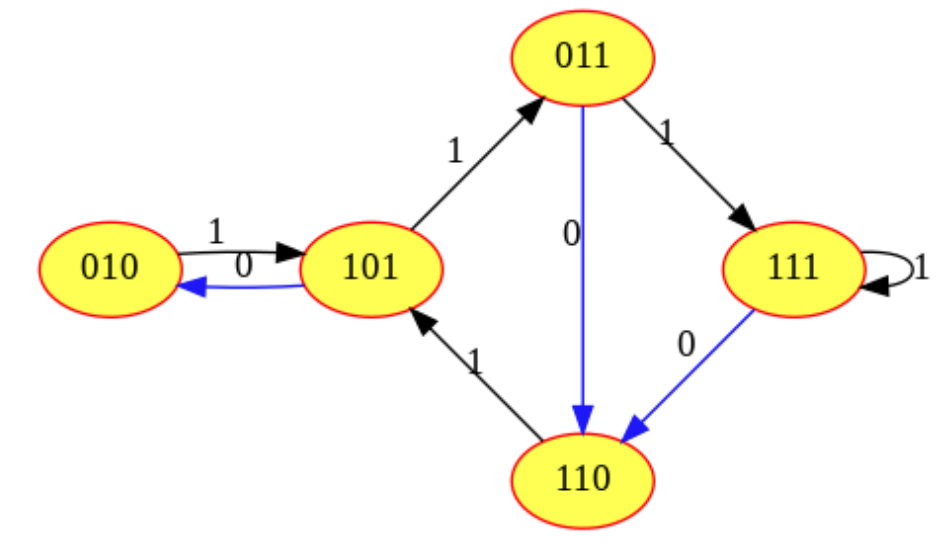
\includegraphics[scale=0.25]{fig/RdB41.png}
    \caption{$(4,1)$-RdB graph.}
    \label{fig:RdB_4_1}
\end{figure}

Denote the $(k,s)$-RdB graph to be $G_{k,s} = (V^{k-1,s},E^{k,s})$, where $V^{k-1,s}$ is the set of all vertices and $E^{k,s}$ is the set of all edges. The following lemmas determining the cardinality of $V^{k-1,s}$ and $E^{k,s}$

\begin{lemma}[\textbf{Number of vertices}]\label{lem:num_V}
    \begin{align}
        \card{ V^{k-1,s}} = \card{ W(k,s)}\label{eq:num_V}
    \end{align}
\end{lemma}
\begin{proof}
    This proof is deduced directly from the construction of $G_{k,s}$ since its set of all vertices is the set of all length $k-1$ sequences containing at most $s$ consecutive letters $0$. 
\end{proof}

\begin{lemma}[\textbf{Number of edges}]\label{lem:num_edges}
    \begin{align}
        \card{ E^{k,s}} = \card{ W(k,s)}\label{eq:card_of_E}
    \end{align}    
\end{lemma}
\begin{proof}
    Observe that for both $\bfx, \bfy\in W(k-1,s)$, if there is an edge from vertex $\bfx = (x_{1},\ldots,x_{k-1})$ to vertex $\bfy = y_{1},\ldots,y_{k-1}$, then $(x_{1},\ldots,x_{k-1},y_{k-1})\in W(k,s)$. 
    
    Besides, for each $s$-RLL sequence $\bfx=(x_{1},\ldots,x_{k})\in W(k,s)$, its prefix and suffix, $(x_{1},\ldots,x_{k-1})$ and $(x_{2},\ldots,x_{k})$, are both $s$-RLL sequence of length $k-1$. Hence, they represent two vertices in the graph $G_{k,s}$ and their connecting edge is represented by the sequence $\bfx$.
    
    So, there is $1-1$ correspondence between $E^{k,s}$ and $W(k,s)$. This results in $\card{ E^{k,s}} = \card{ W(k,s)}$.
\end{proof}

\begin{example}
    According to lemma \ref{lem:num_V} and lemma~\ref{lem:num_edges}, $(4,1)$-RdB graph has $\card{V^{3,1}}=\card{W(3,1)}=5$, and $\card{E^{4,1}} = \card{W(4,1)}=8$. These results can be verified by counting the number of vertices and edges in figure~\ref{fig:RdB_4_1}.
    % Applying lemma \ref{lem:num_V} and lemma~\ref{lem:num_edges} for $k=4,s=1$ gives $\card{V^{3,1}}=\card{W(3,1)}=5$, and $\card{E^{4,1}} = \card{W(4,1)}=8$. Counting the number of edges and vertices in figure~\ref{fig:RdB_4_1} provides the same results
\end{example}

Let $u=(u_{1},u_{2},\ldots,u_{k-1})$ and $v=(v_{1},v_{2},\ldots,v_{k-1})$ be arbitrary vertices in RdB graph. Starting at $v$, the following sequence of edges' labels $(1,u_{1},u_{2},\ldots,u_{k-1})$ apparently forms a proper path going from $v$ to $u$ in RdB graph. Similarly, the sequence of edges' labels $(1,v_{1},v_{2},\ldots,v_{k-1})$ beginning at $u$ is also a directed path from $u$ to $v$. This is sufficient to conclude that the connectivity of RdB graphs is preserved.


% \section{Overview}

% Phần này mô tả tổng quan giải pháp gồm những bước chính nào, hoạt động ra sao. Mục tiêu của phần này là cho người đọc một cái nhìn tổng thể về giải pháp. Để cho dễ hiểu thì nên có một biểu đồ mô tả luồng hoạt động của giải pháp đề xuất. 

% \section{Tên của nội dung chi tiết thứ 1}
% Tên của các chương này đặt theo nội dung mà sinh viên sẽ trình bày trong từng chương. 

% Các chương tiếp theo mô tả chi tiết về các bước, các thuật toán trong giải pháp đề xuất. Có thể trình bày pseudocode cho từng bước. Chú ý, pseudocode chỉ có tác dụng làm chi tiết hoá giải thuật chứ không thay thế được phần thuyết minh về giải thuật. Đối với những chi tiết kỹ thuật khó hiểu nên có các hình minh hoạ để người đọc dễ hiểu. Mỗi một thuật toán/bước thực hiện nên tách ra thành một chương. 

% \section{Tên của nội dung chi tiết thứ 2}

